\documentclass[10pt,twocolumn]{IEEEtran}

\usepackage{ucs}
\usepackage[utf8]{inputenc}
\usepackage{xcolor}
\usepackage{fontenc}
%\usepackage[showframe]{geometry}
\usepackage{graphicx}
%\usepackage{multicol}
%\usepackage{lipsum}
\usepackage{minted}
\usemintedstyle{monokai}
\usepackage[dvips]{hyperref}

%\author{Aravind}
\title{I2C Protocol}
\date{02/05/2017}
 
\begin{document}
  With \verb!\_!:
  \maketitle
   \paragraph{The physical I2C bus}
\newline
SCL is the clock line. It is used to synchronize all data transfers over the I2C bus. SDA is the data line. The SCL & SDA lines are connected to all devices on the I2C bus.

\subparagraph{Masters and Slaves}
\newline
The devices on the I2C bus are either masters or slaves. The master is always the device that drives the SCL clock line. The slaves are the devices that respond to the master. A slave cannot initiate a transfer over the I2C bus, only a master can do that. There can be, and usually are, multiple slaves on the I2C bus, however there is normally only one master.Slaves will never initiate a transfer. Both master and slave can transfer data over the I2C bus, but that transfer is always controlled by the master.

\begin{figure}[p][t]
  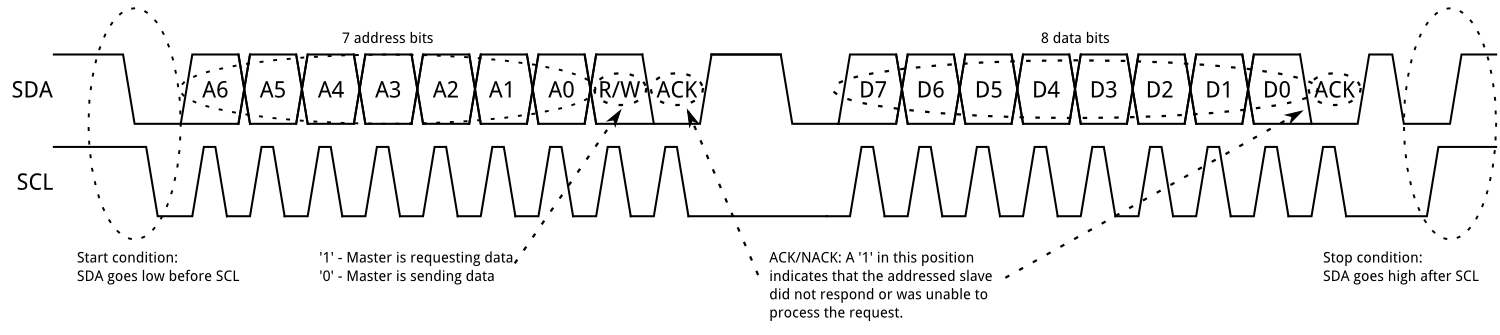
\includegraphics[width=\textwidth]{i2c_concept.png}
  \label{Figure 1: The I2C protocol}
\end{figure}


\paragraph{The I2C Physical Protocol}
\newline
Data is transferred in sequences of 8 bits. The bits are placed on the SDA line starting with the MSB (Most Significant Bit). The SCL line is then pulsed high, then low.For every 8 bits transferred, the device receiving the data sends back an acknowledge bit, so there are actually 9 SCL clock pulses to transfer each 8 bit byte of data. If the receiving device sends back a low ACK bit, then it has received the data and is ready to accept another byte. If it sends back a high then it is indicating it cannot accept any further data and the master should terminate the transfer by sending a stop sequence. 

\subparagraph{I2C Device Addressing}
\newline
Here the I2C address is made of 7 bits. When sending out the 7 bit address, we still always send 8 bits. The extra bit is used to inform the slave if the master is  writing to it or reading from it. If the R/W bit is '0' the master is writing to the slave. If the bit is '1' the master is reading from the slave. The 7 bit address is placed in the upper 7 bits of the byte and the Read/Write (R/W) bit is in the LSB (Least Significant Bit).

\subparagraph{Theory of Operation}
\newline
The I2C master we implemented uses the state machine depicted in Figure 1 to implement the I2C-bus protocol. Upon start-up, the component immediately enters the ready state(here, enters and remains in idle state till an edge trigger happens). 

Once an edge trigger happens the start state generates the start condition on the I2C bus, and the command state communicates the address(start\_addr\_tx) and rw command to the bus. 

The slv\_ack1 state(slave\_hit\_addr) then captures and verifies the slave’s acknowledgment(ack\_one), if not acknowledged goes back to idle state. 

Depending on the rw command, the component then proceeds to either write data to the slave (wr state) or receive data from the slave (rd state). 
In our implementation, we have dealt with write only. If it hits read,it goes back to idle state.

Once state\_reg hits write, it will keep receiving bits of data to write to slave till bit\_cnt reaches 7 (8 bits of data sent).

Once bit\_cnt equals 8, depending on the acknowledgment we receive from slave\_hit\_data , the state either ends the process (ack\_two =0) or goes back to idle state(ack\_two =1). 

Once the process has finished running successfully (i.e. ack\_two =0) it goes back to idle state and waits for the edge trigger (sda). If sda is received as 1, then our I2C repeats the process over again from start.
  
  
  
  \begin{minted}[
    frame=lines,
    framesep=2mm,
    bgcolor=LightGray,
    fontsize=\footnotesize,
    linenos
  ]{vhdl}
-----------------
----code here
-----------------
  \end{minted}

\end{document}


